\section{Theroritical Background}
\subsection{QD 'Artificial Atoms'}
Self-assembled quantum dots (QDs) are localized nano-scale semiconductor structures that creates a three-dimensional(3D) potential well, both in the valence and conduction bands,which trap charge carriers. Due to their small confinement length relative to the particle's wavelength, the energy levels of the QD are quantized with properties similar to atoms which lead them to be described as "Artificial Atoms" \cite{Kastner1993}. \\
In recent years, semiconductor QDs were thoroughly investigated as technology-compatible single photon sources, providing a quantum source of "flying qubits" on demand.\cite{Dekel2000,Michler2000,Michler2000_1,Yuan2002} Moreover, recently, it has been shown that QDs can emit pair of entangled photons \cite{Akopian2006,Hafenbrak2007} and that an emitted photon can be entangled with the remaining spin in the QD. \cite{Pelk2012,Schaibley2013,Gao2012} These achievements form the required building blocks for quantum information processing. \cite{DiVincenzo1998,Duan2001}\\
\subsection{Entangled photons}
\subsubsection{Definition of Entanglement}
Quantum entanglement is a phenomenon in quantum mechanics where two or more particles can become correlated in such a way that the state of each particle cannot be described independently of the state of the others. 
 In other words, The overall state cannot be expressed as a product of the states of their individual subsystems. In other words, an entangled system is one that is not separable.\\
 If, on the other hand, the system is prepared in a separable state, then the overall state can be expressed as a product of the states of the individual particles. In this case, the particles are not entangled, and their states can be described independently of each other.
\subsubsection{The role of entangled photons in quantum information}
Entanglement is a crucial resource in quantum information processing, enabling key advantages over classical information processing and making possible many of the most exciting and promising applications of quantum technologies.
\subsubsection{Fundamental excitations in QD}
In semiconductor QDs, at low temperatures, the basic optical excitation, in which an electron is optically excited from the full valence band, thereby leaving there a hole, to the empty conduction band, is called a bright exciton(BE). In self-assembled QDs, the BE consists of an electron-heavy-hole pair. This optical excitation preserves the spin orientation of the excited electron, and therefore, the electron and hole are said to have anti-parallel spins. The total angular momentum projection of the BE on the direction of the exciting light is, therefore ±1 (like that of the absorbed photon), reflecting the orbital momentum difference between the electron in the valence band to that in the conduction band.
If the excited conduction electron's spin projection is in addition opposite to the spin projection of the ground valence band electron, the electron, and the 2 holes have parallel spins, with a total angular momentum projection of ±2. This type of excitation is optically forbidden since the light electric field cannot change the electronic spin; therefore, it is called dark exciton (DE). Excitons in the QD can also be generated while the QD contains additional charges, such as a single electron or a single hole. Similarly, many other types of multiple carrier configurations can populate the QD at a given time. For example, a biexciton is two excitons (two electrons and two holes), and a positively (negatively) charged exciton (trion) is an exciton with the addition of one hole (electron), just to mention a few basic QD excitations.
\subsubsection{The $\Lambda$ and $\Pi$ systems}
$\Lambda$ system is a three level physical system in which the two eigenstates of a qubit are connected to a third auxiliary level via an optical transition. An example of a relevant to this proposal Λ system is presented in Figure $\ref{fig:PiSystem}$(a),where the two (degenerate) BE eigenstates are coupled to the ground (nondegenerate) biexciton state. Similarly, one can also think about the BE and the (non-degenerate) vacuum level as an Inverted Λ system, or a V system (not shown). 
\begin{figure}[H]
	\centering
	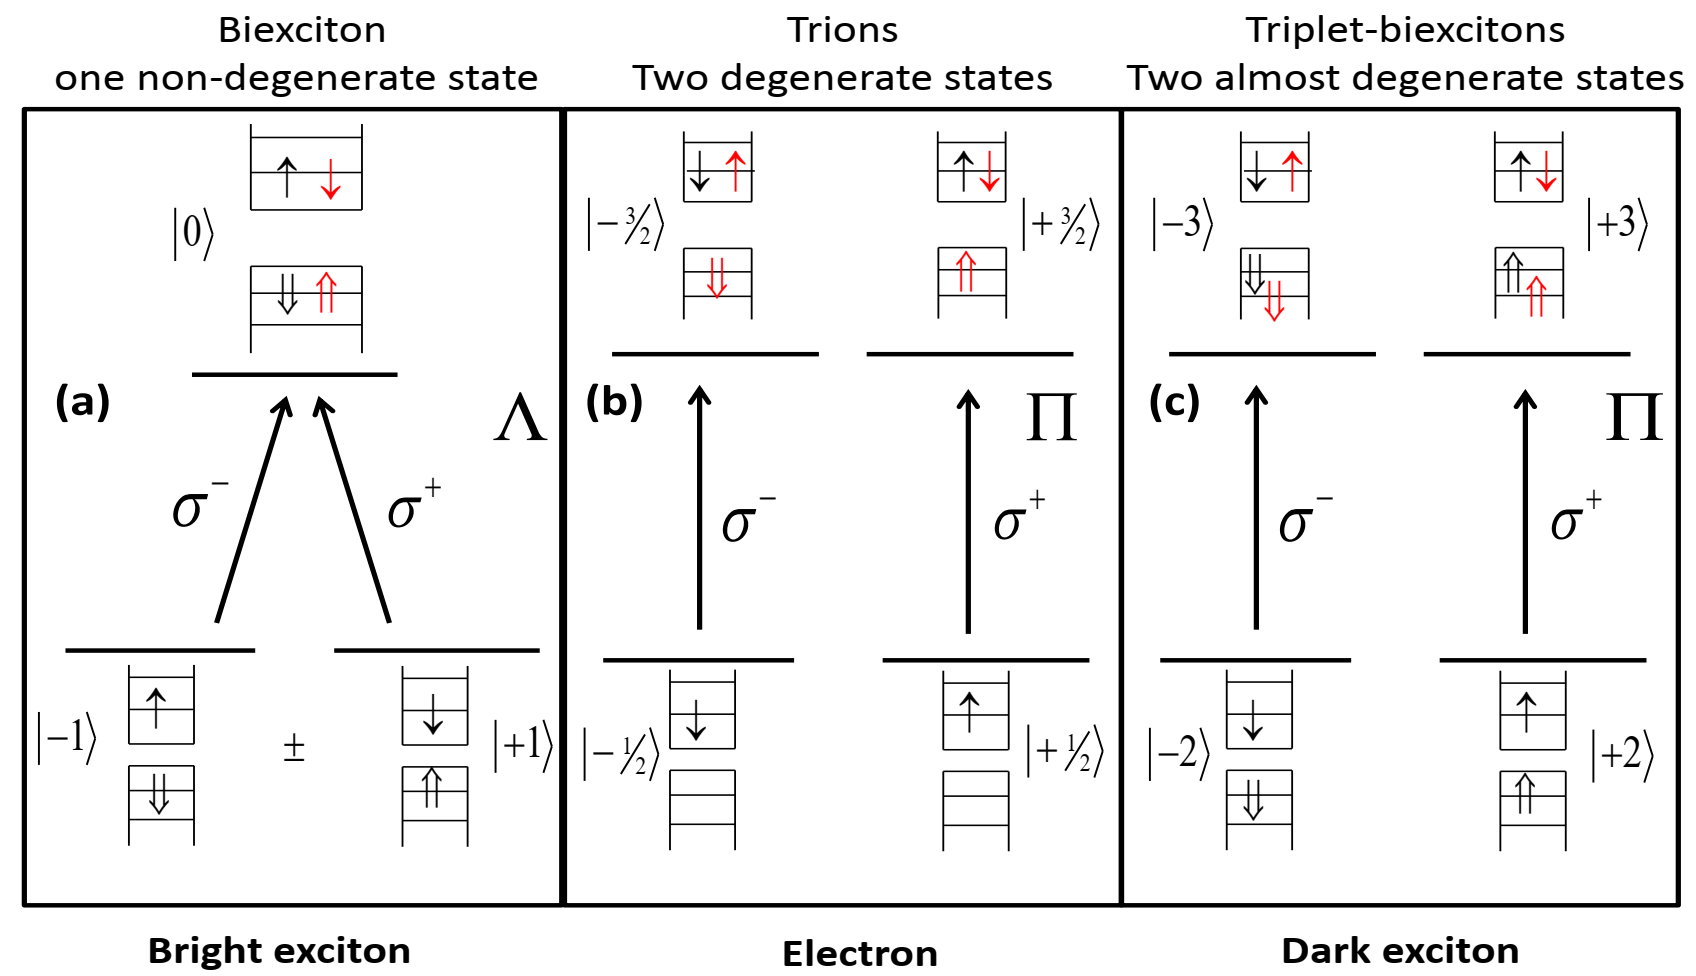
\includegraphics[scale=0.32]{figures/pISystem.png}
	\caption{Schematic description of the energy level and selection rules for
optical transition in Λ and Π systems. (a) A Λ system formed by the BE and
the ground biexciton. (b) A Π system formed by a (degenerate) electron spin
qubit and excited trion states. (c) A Π system formed by the (degenerate) DE
qubit and an excited biexciton states. The states are described by their total
angular momentum projections. The arrows symbolize optical transitions
and σ+ (σ-) symbolizes right (left) hand circular polarization.}
	\label{fig:PiSystem}
\end{figure}
\subsubsection{QD as a source of single photon}
\subsubsection{exciton-biexciton cascade (QD as a source of entangled photon pair)}
\subsubsection{QD spin as a generator for a string of entangled photons}
\subsection{Optimized Platforms for the emission from a QD (Grating/Open Cavity)}
